\chapter{State of the Art}
\label{stateoftheart}
\thispagestyle{empty}

\begin{quotation}
{\footnotesize
\noindent{\emph{``Morty: I just I didn't get a lot of sleep last night. Maybe my dreams were just too loud or something.\\
Summer: Or maybe you were out all night again with Grandpa Rick. \\
Jerry: What? \\
Beth: Dad? \\
Rick: What, so everyone's supposed to sleep every single night now? You realize that nighttime makes up half of all time?''}}
\begin{flushright}
Rick and Morty (Season 1, Episode 1)
\end{flushright}
}
\end{quotation}


\vspace{0.5cm}

Many real-world problems are inherently hierarchically structured, meaning that it is possible look at a complicated challenge as a sequence of its more manageable components. As humans, we  tend to learn new tasks by breaking them up into easier ones and ordering them. A very simple real world example can be having a cup of coffee. The subtasks for this goal would be pouring the coffee, adding sugar, adding milk, and stirring. 

Artificial intelligence researchers benefited of this structure to afford clarity, concision and implementation hided in large scale tasks, using various ways of abstraction. Macros or macro operators form the fundamentals of the hierarchical notion in AI research. They can be used to group a whole series of actions into one and can be called as one primitive action. In addition, in the definition of a macro another macro can be defined. 

\section{Hierarchy in control systems}
\begin{figure}[t]
      \centering
      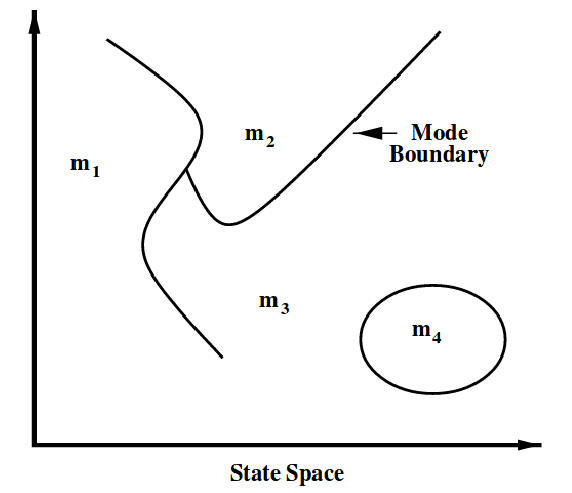
\includegraphics[width = 0.5\textwidth]{./pictures/modeswitching.png}
      \caption{Mode switching control}
      \label{fig:modeswitching} 
\end{figure}

In control theory, abstraction plays an important role. One way to implement the abstraction and hierarchy is to use hybrid systems. Hybrid systems are dynamical systems that exhibit both continuous and discrete dynamic behavior. When a control system is designed exploiting the hybrid formalism, typically, discrete controllers are in the higher levels of the hierarchy. This part is analogous to macros in AI research. In control theory, discrete action with respect to the state information is applied, and this action remains effective for an extended time. That is, discrete action changes the dynamics of the underlying controllers that act with continuous dynamics.

In AI terms a macro is called according to the state and it stays active until it terminates. Hybrid systems are a compromise between centralized and decentralized control schemes. In the centralized control scheme, the control signal is computed with the information from the entire system and then it is distributed to all the actuators. Despite its obvious advantages, such as having the possibility of global optimization, it is not practical as it requires high computational resources and the design tends to get tedious in large scale problems. In a completely decentralized control scheme, local controllers undertake the computation of commands for the subsystem actuators having limited information from the plant. Unlike the prior, they are easy to design. However, in cases of strong couplings between subsystems and/or where the closed-loop performance is crucial, this scheme is not adequate. When a decentralized solution cannot be accepted and a completely centralized solution is too expensive, a compromised scheme with some form of multilevel hierarchy is convenient. In the resulting systems, lower level deals with the local aspects of the performance whereas the higher level is responsible for the global criteria. In such hierarchy, the two levels possibly need different models of the plant. Local controllers need more detailed information on the dynamics of the part they act on and often they work with continuous models while for the higher level such details are impractical to handle. Thus, the typical choices for the higher level are discrete models. 

Mode switching controllers are a class of hybrid systems, where the control law depends on the location in state space, as in Figure~\ref{fig:modeswitching}. In other words, the higher level controller in the hierarchy switches between low level controllers according to the observation of the state. Mode switching controllers are commonly used in many control applications in order to allow relatively simple controllers to be used in different operating regimes, such as aircraft climbing steeply vs. cruising at constant elevation.
In~\cite{Grudic2000LocalizingSI}, the agent’s policy is designed as a deterministic mode switching controller and a new type of reinforcement learning called Boundary  Localized  Reinforcement Learning (BLRL) is proposed.

\section{Hierarchy in Reinforcement Learning}

Boundary  Localized  Reinforcement Learning (BLRL) is one of the many ways of defining a policy for a subset of a state in reinforcement learning. Examples of other forms of partial policies can be given as temporally-extended actions, options~\cite{Sutton1999BetweenMA}, skills~\cite{Thrun1994FindingSI} and behaviors~\cite{Brooksbehaviors, Huber1997AFC}. The idea of partial policies with well defined termination conditions is one of the key methods of temporal abstraction introduced to reinforcement learning to improve the scalability and enhance the performance. 

The nature of Markov decision processes (MDP), the models on which RL is based, does not involve actions that persist for an amount of time or, simply, temporally extended actions. In the classical MDP framework, an agent perceives the state of its environment at some discrete time t, takes an action accordingly, and, at the next time step t+1, gets from the environment a reward and the information about the next state s'. Moreover, the environment dynamics can be expressed with a transition function, which returns the probability of passing to state s’ given the current state s and the action a. Extension of the idea of higher level actions that contain lower level actions, which may or may not be the conventional one step actions, results in another type of decision process: semi-Markov decision process (SMDP). For SMDPs, the waiting time in state s upon the execution of action a is a variable and it represents relevant information. It corresponds to the execution time of a high-level action and depends on the policies and the termination conditions of all the lower-level ones. An SMDP consists of a set of states, a set of actions, an expected cumulative discounted reward for each state-action pair and a well-defined joint distribution of the next state and transit time. All three methods for introducing temporal extensions to actions that will be presented in this section, to explore the interaction between MDPs and SMDPs.

\subsection{Options}

An option is a temporally extended action with well defined policy. The term "option" is a generalization of primitive actions to adapt to the concept of temporal extension in SMDPs. In other words, an MDP  which has options instead of primitive actions is an SMDP. Figure~\ref{fig:options} from~\cite{Sutton1999BetweenMA} illustrates this definition. As mentioned above, the state trajectory of an MDP consists of small, discrete-time transitions, whereas that of an SMDP covers larger, continuous time transitions. Options enable an MDP trajectory to be analyzed in either way.
\begin{figure}[t]
      \centering
      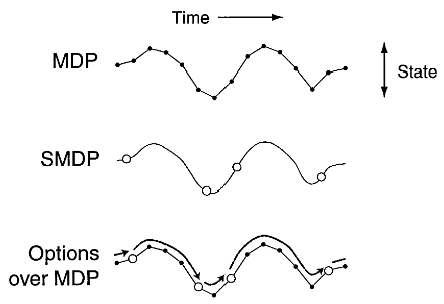
\includegraphics[width = 0.6\textwidth]{./pictures/options.png}
      \caption{Options over MDPs}
      \label{fig:options} 
\end{figure}
The main reason for the construction of options is to express temporally-extended actions in reinforcement learning and thus potentially increase the speed of learning in large-scale problems, particularly at the initial steps. Options can also assist the transfer of learning information between different tasks. For instance the option grab-the-door-knob whose policy is learned in open-the-door task might as well be used in close-the-door task. Though this advantage is highly dependent on the design of the options. This framework also facilitates adding prior knowledge to design. The designer of an RL system typically uses prior knowledge about the task to add a specific set of options to the set of available primitive actions.
An option has three components: a policy $\pi : \mathcal{S}^+\times\mathcal{A} \rightarrow \left[0,1\right]$, a termination condition $\beta: \mathcal{S} \rightarrow \left[0,1\right]$ and an initiation set $I \in \mathcal{S}$. An option is available only in the states that are contained in its initiation set. An option can be selected according to the policy over the options. If an option is selected, the policy of that option is followed until the option is terminated. The probability of an option to terminate in state s is given by $\beta(s)$. If the option does terminate, the agent gets to choose either a primitive action or another option that is available at the termination state of the previous one. Indeed, a primitive action can be considered as an option, called one-step option with $I=\{s: a \in \mathcal{A}_s\}$ and $\beta(s) = 1$ for all $s$. Each option can select another option, and so on, until one-step options are selected that correspond to the actions of the core MDP which leads to a hierarchical structure

\subsection{Hierarchy of Abstract Machines}

A machine is a partial policy represented by a Finite State Automaton. A Hierarchy of Abstract Machines (HAM)~\cite{Parr1997ReinforcementLW} is formed by the start of the execution of an initial machine and the termination of all the machines reachable from the initial one. Machines for HAMs are defined like programs that execute based on their own states, which can be of 4 types: \textit{action, call, choice} and \textit{stop}. In the \textit{action} states an action executes in the MDP. \textit{Call} sates, instead, start the execution of another machine. In \textit{choice} states, the next state of the machine is selected stochastically. \textit{Stop} halts the machine and returns the control to the previous call state. Apart from the set of states, a transition function and a start function which determines the initial state of the machine are needed in order to specify a machine. The transition function of a machine is defined as a stochastic function that depends on the current machine state and some features of the environment state and it determines the next state of the machine after an \textit{action} or a \textit{call} state. 

The interaction of a HAM $\mathcal{H}$ with an MDP $\mathcal{M}$ yields an induced MDP $\mathcal{H}\circ\mathcal{M}$. $\mathcal{H}\circ\mathcal{M}$ is indeed an MDP itself, with state set $\mathcal{S} = \mathcal{S}_M \times \mathcal{S}_H$, where $\mathcal{S}_M$ is the set of states of $\mathcal{M}$ and $\mathcal{S}_H$ is the set of states of $\mathcal{H}$. It is important to note that when we try to determine the optimal policy of $\mathcal{H}\circ\mathcal{M}$, the only relevant points are the \textit{choice} points. This is because, when $\mathcal{H}$ is in a state that is not a \textit{choice} state, only one action is allowed. These states can be eliminated to produce an SMDP called $\mathit{reduce}(\mathcal{H}\circ\mathcal{M})$. The optimal policy for $\mathcal{H}\circ\mathcal{M}$ will be the same as that of this SMDP, which, in turn, may increase the policy iteration speed. The above-mentioned property is particularly useful for RL. HAM constraints can reduce significantly the exploration effort by reducing the state-space in which the agent operates.

Options expand the repertoire of actions by defining the conventional primitive actions as a special form of options called one-step options, whereas HAMs are designed to constrain the set of allowed actions. For instance, in a case where an agent can choose up, down, right and left as actions, a machine may dictate “repeatedly choose right or down”. Such a command would erase the policies that choose  going up or left, which in return would simplify the MDP.

\subsection{MAX-Q Value Function Decomposition}
Another approach to HRL is the MAX-Q value function decomposition, developed in~\cite{Dietterich2000HierarchicalRL}. MAX-Q decomposes the value function of the main MDP into an additive combination of the value functions of the sub-MDPs.

To do so, MAX-Q takes an MDP $\mathcal{M}$ and decomposes it into a finite set of subtasks ${\mathcal{M}_0, \mathcal{M}_1, \mathcal{M}_2,\dotsc,\mathcal{M}_n}$. Here $\mathcal{M}_0$ refers to the root subtask. Once the root subtask is achieved the task itself is achieved. A subtask is formalized by a tuple $\langle \mathcal{T}_i, \mathcal{A}_i, \tilde{\mathcal{R}}^{i}\rangle$ where $\mathcal{A}_i$ is a set of admissible actions to achieve the subtask,$\mathcal{T}_i$ is a termination predicate that partitions the MDP states $\mathcal{S}$ into a set of active states $\mathcal{S}_i$ and a set of terminal states $\mathcal{A}_i$. A subtask can execute only in the states $s\in\mathcal{S}_i$ and once $\mathcal{M}$ goes into one of the states in $\mathcal{T}_i$, the subtask terminates. $\tilde{\mathcal{R}}^{i}$ is a deterministic pseudo-reward for each transition to a terminal state. By definition, $\mathcal{R}^{*i}$ is zero anywhere outside the terminal states. If the terminal state is the goal state, typically the pseudo-reward is zero again and for other terminal states it is negative. Each primitive action is a special case of subtask, as it was with options. $\mathcal{T}_i$ of a primitive action is that it terminates directly after the execution, $\tilde{\mathcal{R}}^{i}$ is uniformly zero and $\mathcal{A}_i$ contains a. For each subtask $\mathcal{M}_i$, a policy $\pi_i$ is defined. The hierarchical policy for the root task $\mathcal{M}_0$ is $\pi = \left\{\pi_0,\dotsc, \pi_n\right\}$. MAX-Q executes the hierarchical policy as the ordinary programming languages executes subroutines, using a stack discipline. That is, it explicitly defines a pushdown stack. Let us denote the contents of this stack at time t as $\mathcal{K}_t$. Once a subtask is active, its name and parameters are pushed up in the stack and once it terminates it is aborted from the stack together with everything that was above. 

Unlike the other two approaches, in this algorithm, the flow of information is from lower-level subtasks to higher-level subtasks only, and not vice versa. Due to this unidirectional flow of information, the decisions taken at a lower level will be independent of the higher-level goal to be achieved. It is easy to see that due to this additional restriction, the policies produced by this approach may not be hierarchically optimal but \textit{recursively optimal}. Recursive optimality is that the policy at each level is optimal assuming that policies of all lower levels are fixed. In general, a recursively optimal policy may not be hierarchically optimal and vice versa. A hierarchically optimal policy will always be at least as good as a recursively optimal one.

The idea of hierarchical policy is familiar from the discussion about the options. The policy over options, corresponds to that of the subtask in MAX-Q. In addition to that, the termination condition beta of the options framework translates to the termination predicate in MAX-Q. In this case, $\beta$ can only take the values  0 or 1 instead of a continuous interval between 0 and 1.

\section{Policy Search Methods}
Reinforcement learning in robotics is challenging, mainly due to the continuous action and state spaces. One technique to address this problem is discretization. However, particularly when considering actions with high dimensionality when a fine control action is needed, this approach becomes impractical. Most value-based reinforcement learning methods need to work on discrete actions, as they  estimate a value for state-action pairs and use the estimated values to build the policy: to produce a policy they need to search the action with the best value at each state, that can become impractical, unless the action set is discrete. 

An alternative to value-based methods is Policy search (PS).
PS methods start with a parameterized policy and try to find the parameters trough evaluating trajectories until a locally optimal solution is found. In robotics tasks, it is relatively simple to describe a family of suitable policies. Moreover, starting with a parameterized policy gives the opportunity to encode prior knowledge. Continuous action spaces are not an issue for PS, as the action is produced by the policy parametrization and no maximization of the action-value function is needed. For this reasons PS methods are frequently used in robotics. 

However, unlike value-based approaches, policy search might not converge to the global optima. In addition, they tend to converge slower than the value-based methods.

To take advantage from both PS and value-based approaches, Actor-critic algorithms where developed. Figure~\ref{fig:pstovaluebased} depicts these algorithms on the gray scale between purely value-based and purely policy search-based methods

\begin{figure}[t]
	\centering 		
    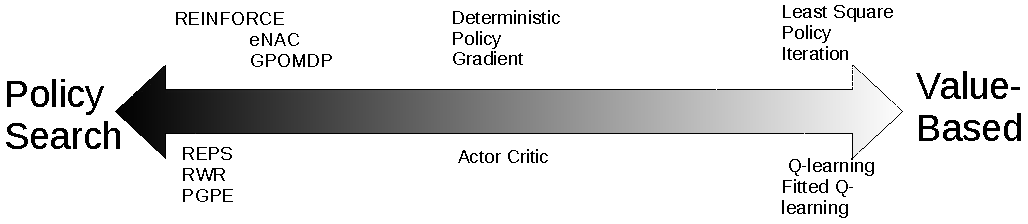
\includegraphics[width=\textwidth]{./pictures/greyscale.pdf}
    \caption[policy search, actor critic and value-based]{algorithms on a gray scale from direct policy search to value-based. Actor critic algorithm are in the middle.}
    \label{fig:pstovaluebased} 
\end{figure}


There are two ways of approaching PS: model-based and model-free. Model-based policy search addresses this problem by first learning a simulator of the robot’s dynamics from data. Subsequently, the simulator generates trajectories that are used for policy learning. It is interesting to note here that the differences between the adaptive control and the model-based policy search are indeed subtle. They both start with a class of models and predict a forward-model. When the interaction with the real robotic environment is difficult, due to safety or time constraints, model-based approaches are a preferable solution.

Model-free PS methods update the policy directly based on sampled trajectories and the obtained immediate rewards for the trajectories. Model-free PS methods try to update the parameters such that trajectories with higher rewards become more likely when following the new policy. Since learning a policy is often easier than learning an accurate forward model, the model-free approach is more used. 

The policy updates in both model-free and model-based policy search are based on either policy gradients (PG), expectation–maximization (EM) based updates, or information-theoretic insights (Inf.Th.). 

\subsection{Policy gradient}
With this method, parameters are updated with a gradient ascent so as to maximize the expected return, $\mathcal{J}_\theta$. The direction of the update is determined by the gradient $\nabla_\theta\mathcal{J}_\theta$. There are several ways to estimate this gradient. The simplest one of them is the finite difference method. The basic idea behind this method is to slightly perturb the parameters, $\delta\theta$, and examine the change in the reward, $\delta R$. The second method uses the likelihood-ratio approach: $\Delta p_\theta(y)=p_\theta(y)\Delta\log p_\theta(y)$. Likelihood ratio methods can be step-based or episode-based. Examples of step-based likelihood ratio methods are REINFORCE~\cite{Williams1992SimpleSG}, Gradient Partially Observable MDP (GPOMDP)~\cite{Baxter1999DirectGR, Bartlett2001InfiniteHorizonPE}. In REINFORCE and GPOMDP  algorithms the exploration is step-based, i.e., perturbation is applied to the actions at every time-step. Instead, Policy Gradient with Parameter Exploration Algorithm (PGPE)~\cite{Sehnke2008PolicyGW}, the exploration is done over the parameters, i.e., the perturbation is applied to the parameters at the beginning of the episode. The third method is based on the natural gradient. The key concept behind the natural gradient is to measure the distance between the distributions using the Kullback–Leibler divergence (KL) instead of using the euclidean distance between distribution parameters, to achieve a stable learning behavior. To achieve this goal natural gradient uses Fisher information matrix as metric. In this way, the gradient computed is invariant to the re-parametrization of the same policy, making the natural gradient also invariant to scale changes of the parameters. The computed gradient is rotated less than 90 degrees, therefore the same convergence properties of the vanilla gradient applies. Episodic Natural Actor Critic (eNAC)~\cite{Peters:2008:NA:1352927.1352986} is one of the algorithms that exploit this idea. 

\subsection{Expectation-Maximization (EM)}

The EM-based approach aims at making actions with high future reward more likely. EM formulates the policy search as an inference problem. The trajectories $\tau$ are the latent variables in the model and the observed value is the reward event. Then the classical EM algorithm is used to infer the new policy. Unlike the PG methods, since for most of the used policies there is a closed-loop solution, there is no need to determine a learning rate, which is a tricky task as it may lead to slow convergence or unstable policies. On the other hand, EM neglects the influence of the policy update on the trajectory distribution which can cause another problem: large jumps in the policy. It changes the behavior abruptly and there is a possibility that this new behavior may be extremely far from the optimal one, even damage the robot. Policy learning by Weighting Exploration with the Returns (PoWER)~\cite{Kober2008PolicySF} and Reward-Weighted Regression (RWR)~\cite{Peters2007ApplyingTE} are among the algorithms using this approach. PoWER uses episode-based exploration strategies with step-based evaluation strategies. PoWER is similar to episodic RWR but it has a more structured exploration strategy.

\subsection{Information Theoretic Approach (Inf. Th.)}
Information theoretic insight is exploited in Relative Entropy Policy Search (REPS)~\cite{Daniel2012HierarchicalRE, Peters2010RelativeEP}. It combines the advantages of two approaches described above. Instead of following the gradient, REPS formulates the policy update as an optimization problem. It tries to find the policy parameters that maximizes J while keeping bounded the KL w.r.t. the previous parameters. 

Using maximum likelihood estimates for the parameter updates is also beneficial for learning multiple solutions, as we can represent them with a mixture model. REPS can be extended to learning multiple solutions by reformulating the problem as a latent variable estimation problem, where the high level options are latent variables. The resulting algorithm is the Hierarchical Relative Entropy Policy Search (HiREPS)~\cite{Daniel2012HierarchicalRE} algorithm. 


\section{Hierarchical Policy Gradient Algorithm}

As discussed above, policy gradient algorithms are convenient for complex robotics tasks with high dimensions and continuous action spaces. However, they tend to suffer from slow convergence due to large variance of their gradient estimators. Hierarchical reinforcement learning methods gained the interest of researchers as a means to speed up learning in large domains. \cite{GhavamzadehHierarchicalPG} combines the advantages of these two and proposes hierarchical policy gradient algorithms (HPG). 

HPG objective is to maximize the weighted reward to go similar to~\cite{Marbach1998SimulationB} or~\cite{Bartlett2001InfiniteHorizonPE}. As the flat policy gradient algorithm, HPG searches for a policy in a set that is typically smaller than the set of all possible policies as it is parameterized and converges to local optimal policy rather than the global.  

In order to perform this approach, similarly to MAX-Q, the overall MDP $\mathcal{M}$ is divided into a finite set of subtasks. That is,${\mathcal{M}_0, \mathcal{M}_1, \mathcal{M}_2,\dotsc,\mathcal{M}_n}$ where $\mathcal{M}_0$ is the root task. The state space is divided into initiation and termination state sets for these subtasks and each subtask $\mathcal{M}_i$ that is not a primitive action has a policy $\pi_i$. The hierarchical policy is executed using a stack discipline. \cite{GhavamzadehHierarchicalPG} makes the assumption that the root task is episodic and also models the subtasks as an episodic problem. That is, all terminal states transit to an absorbing state $\ s^{*i}$ with probability 1 and reward 0.

\cite{GhavamzadehHierarchicalPG} suggests another method to speed up learning in HPG, called hierarchical hybrid algorithms in which some of the subtasks are formalized as value function-based reinforcement learning. These subtasks are in the higher levels where the action spaces are usually finite and the state relevant dimensions are fewer.  

Despite the obvious advantages, these algorithms are highly task-specific. That is, they are failing to build up a general framework for hierarchical policy gradient. Indeed the implementation of this algorithm for the ship steering task described in~\cite{GhavamzadehHierarchicalPG} is not trivial. It includes various shifts between different state-action spaces and intricate external reward definitions. Our approach aims to address these issues by implementing a framework that makes the hierarchy design for reinforcement learning more intuitive. 

